\subsection{FFT Filter}\label{sect:fft-filter}

The FFT filter is used to modify the frequency domain of the input sample in
order to better measure the distinct frequencies we are interested in.
Two filters are useful to speech analysis: high frequency boost, and low-pass
filter (yet we provided more of them, to toy around).

Speech tends to fall off at a rate of 6 dB per octave, and therefore the high
frequencies can be boosted to introduce more precision in their analysis.
Speech, after all, is still characteristic of the speaker at high frequencies,
even though they have a lower amplitude.  Ideally this boost should be performed
via compression, which automatically boosts the quieter sounds while maintaining
the amplitude of the louder sounds.  However, we have simply done this using a
positive value for the filter's frequency response.
The low-pass filter (\xs{sect:low-pass}) is used as a simplified noise reducer, simply cutting off
all frequencies above a certain point.  The human voice does not generate sounds
all the way up to 4000 Hz, which is the maximum frequency of our test samples,
and therefore since this range will only be filled with noise, it may be better
just to cut it out.

Essentially the FFT filter is an implementation of the Overlap-Add method of FIR
filter design \cite{dspdimension}.  The process is a simple way to perform fast convolution, by
converting the input to the frequency domain, manipulating the frequencies
according to the desired frequency response, and then using an Inverse-FFT to
convert back to the time domain. \xf{fig:fft-filter} demonstrates
the normalized incoming wave form translated into the frequency domain.

\begin{figure}
	\centering
	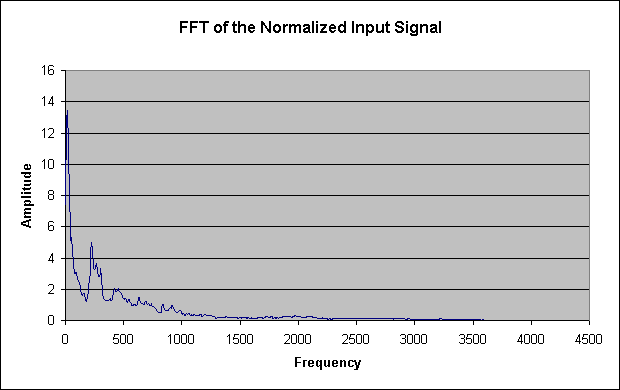
\includegraphics[width=400pt]{../graphics/graphs/fft.png}
	\caption{FFT of normalized aihua5.wav from the testing set.}
	\label{fig:fft-filter}
\end{figure}


The code applies the square root of the hamming window to the input windows
(which are overlapped by half-windows), applies the FFT, multiplies the results
by the desired frequency response, applies the Inverse-FFT, and applies the
square root of the hamming window again, to produce an undistorted output.

Another similar filter could be used for noise reduction, subtracting the
noise characteristics from the frequency response instead of multiplying,
thereby remove the room noise from the input sample.
